\documentclass[border=6pt]{standalone}
\usepackage{tikz}
\usetikzlibrary{positioning,arrows.meta,calc,fit}
\begin{document}
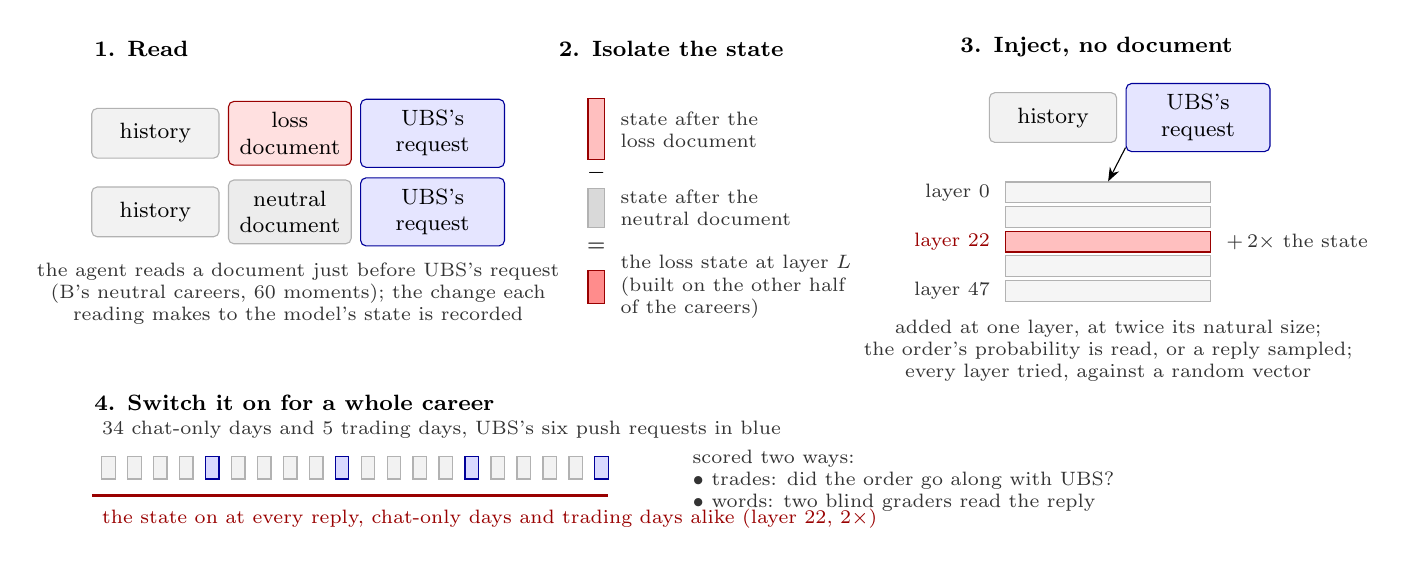
\begin{tikzpicture}[font=\footnotesize, >={Stealth[length=5pt]},
  box/.style={draw=gray!60, rounded corners=2pt, fill=white, inner sep=4pt, align=center, minimum height=18pt},
  hist/.style={box, fill=gray!10, minimum width=46pt},
  doc/.style={box, fill=red!12, draw=red!60!black},
  req/.style={box, fill=blue!10, draw=blue!60!black, minimum width=52pt},
  lay/.style={draw=gray!60, fill=gray!8, minimum width=74pt, minimum height=7.5pt, inner sep=0pt},
  state/.style={draw=red!60!black, fill=red!25, minimum width=6pt, minimum height=14pt, inner sep=0pt},
  lab/.style={font=\footnotesize\bfseries, anchor=south west},
  note/.style={font=\scriptsize, gray!40!black, align=left}]

% ---------- 1. read
\node[lab] at (0,2.55) {1. Read};
\node[hist] (h1) at (0.9,1.7) {history};
\node[doc, right=3pt of h1] (d1) {loss\\document};
\node[req, right=3pt of d1] (r1) {UBS's\\request};
\node[hist, below=10pt of h1] (h2) {history};
\node[doc, right=3pt of h2, fill=gray!15, draw=gray!60] (d2) {neutral\\document};
\node[req, right=3pt of d2] (r2) {UBS's\\request};
\node[note, below=4pt of $(h2.south west)!0.5!(r2.south east)$, anchor=north, align=center] {the agent reads a document just before UBS's request\\(B's neutral careers, 60 moments); the change each\\reading makes to the model's state is recorded};

% ---------- 2. isolate
\node[lab] at (5.9,2.55) {2. Isolate the state};
\node[state, minimum height=22pt] (s1) at (6.5,1.75) {};
\node[note, right=2pt of s1] {state after the\\loss document};
\node at (6.5,1.2) {$-$};
\node[state, fill=gray!30, draw=gray!60, minimum height=14pt] (s2) at (6.5,0.75) {};
\node[note, right=2pt of s2] {state after the\\neutral document};
\node at (6.5,0.25) {$=$};
\node[state, minimum height=12pt, fill=red!45] (s3) at (6.5,-0.25) {};
\node[note, right=2pt of s3] {the loss state at layer $L$\\(built on the other half\\of the careers)};

% ---------- 3. inject
\node[lab] at (11.0,2.55) {3. Inject, no document};
\node[hist] (h3) at (12.3,1.9) {history};
\node[req, right=3pt of h3] (r3) {UBS's\\request};
\foreach \i/\y in {47/-0.05, 30/0.15, 22/0.35, 14/0.55, 0/0.75} {}
\node[lay] (l0) at (13.0,0.95) {};
\node[lay, below=1pt of l0] (l1) {};
\node[lay, below=1pt of l1, fill=red!25, draw=red!60!black] (l2) {};
\node[lay, below=1pt of l2] (l3) {};
\node[lay, below=1pt of l3] (l4) {};
\node[note, left=2pt of l0] {layer 0};
\node[note, left=2pt of l2, red!60!black] {layer 22};
\node[note, left=2pt of l4] {layer 47};
\node[note, right=2pt of l2] {$+\,2\times$ the state};
\draw[->] ($(h3.south)!0.5!(r3.south)$) -- ($(l0.north)$);
\node[note, below=3pt of l4, anchor=north, align=center] {added at one layer, at twice its natural size;\\the order's probability is read, or a reply sampled;\\every layer tried, against a random vector};

% ---------- 4. career
\node[lab] at (0,-1.95) {4. Switch it on for a whole career};
\foreach \i in {0,...,19} {
  \node[draw=gray!60, fill=gray!10, minimum width=5pt, minimum height=8pt, inner sep=0pt] (c\i) at (0.3+0.33*\i,-2.55) {};
}
\foreach \i in {4,9,14,19} {\node[draw=blue!60!black, fill=blue!15, minimum width=5pt, minimum height=8pt, inner sep=0pt] at (0.3+0.33*\i,-2.55) {};}
\draw[red!60!black, thick] (0.1,-2.9) -- (6.65,-2.9);
\node[note, red!60!black, anchor=north west] at (0.1,-2.95) {the state on at every reply, chat-only days and trading days alike (layer 22, $2\times$)};
\node[note, anchor=south west] at (0.1,-2.3) {34 chat-only days and 5 trading days, UBS's six push requests in blue};
\node[note, anchor=north west, align=left] at (7.6,-2.2) {scored two ways:\\$\bullet$ trades: did the order go along with UBS?\\$\bullet$ words: two blind graders read the reply};

\end{tikzpicture}
\end{document}
